\chapter{Analýza}

\section{Alzheimerova choroba \label{sec:ad}}

Alzheimerova choroba je najčastejšou príčinou demencie. Prvotné príznaky tejto choroby sú zhoršenie pamäti, zabúdanie nedávnych udalostí, mien, neschopnosť rozoznávať známe miesta či orientovať sa v čase \cite{Alzheimer.sk_2019}. Jej priebeh sa vyznačuje postupným poklesom kognitívnych funkcií, postupným zhoršením pamäte, myslenia, rozprávania a schopnosti učenia sa \cite{duthey2013background}. Najčastejšie sa vyskytuje u ľudí starších ako 65 rokov, s pravdepodobnosťou výskytu až 50\% po dovŕšení 85 rokov života \cite{duthey2013background}.
% khan2016biomarkers uvadza 24–33%, dafuuuuq???
% Age is the strongest risk factor for LOAD. Epidemiological studies have found that <1% of individuals aged 60–65 years have AD, and the prevalence increas- es exponentially to 24–33% of individuals aged 85 years (Alzheimer’s Disease (AD)–World Health Organization). Another estimate found that among pa- tients affected with AD, 4% are under age 65, 6% are 65–74, 44% are 75–84, and 46% are 85 or older (Alzheimer’s disease facts and figures 2012). The inci- dence of AD increases exponentially with age, and females are disproportionally (2:1) more susceptible to AD compared to male.
S narastajúcim vekom človeka sa zvyšuje pravdepodobnosť ochorenia. Pravdepodobnosť ochorenia zvyšujú taktiež úrazy hlavy, poruchy prekrvenia mozgu, pozitívna rodinná anamnéza či vzdelanie (pretože ľudia s nižším vzdelaním majú väčšie riziko rozvoja tohto ochorenia) \cite{Alzheimer.sk_2019}. Toto ochorenie sa vyskytuje častejšie u žien ako u mužov, v pomere 2:1 \cite{khan2016biomarkers}.

Alzheimerova choroba nie je ``iba`` o strate pamäti, ale aj šiestou najčastejšou príčinou smrti v USA \cite{Figures_2017}. Medzi rokmi 2000 až 2017 sa počet úmrtí v USA viac ako zdvojnásobil \cite{Figures_2017}. Ľudia starší ako 65 rokov ktorým bola diagnostikovaná táto choroba sa v priemere dožívajú 4 až 8 rokov po jej diagnóze \cite{Figures_2017}.

% Spomenut Amyloid beta?

\subsection{Diagnostika Alzheimerovej choroby}

Alzheimerova býva diagnostikovaná kombináciou viacerých ukazovateľov. Pri ur-čovaní diagnózy sa používajú neuropsychometrické (kognitívne) testy, rádiologické snímky (angl. neuroimaging data), biologické ukazovatele a špecifické kritériá, na základe ktorých je možné vylúčenie iných chorôb u pacienta z jeho histórie vývoja ochorenia \cite{khan2016biomarkers}. T. Khan zadefinoval tieto ukazovatele do tzv. komplexného rámca pre diagnózu Alzheimerovej choroby (Obr. \ref{fig:alzheimer_diagnosis_scheme}). V súčastnosti sa v tejto oblasti skúmajú biologické ukazovateľe (ich identifikácia a použitie), keďže používanie (a teda aj vytvorenie) rádiologických ukazovateľov je drahé \cite{khan2016biomarkers} (vyžaduje si to zaškolený personál a vybavenie). Biologické ukazovateľe zatiaľ nie sú dostatočne spoľahlivé \cite{khan2016biomarkers}.
% COMPREHENSIVE ALZHEIMER’S DISEASE DIAGNOSTIC FRAMEWORK, chapter 2.7
% TODO: zadefinoval? dobre slovo?

\begin{figure}[h!]
\centering
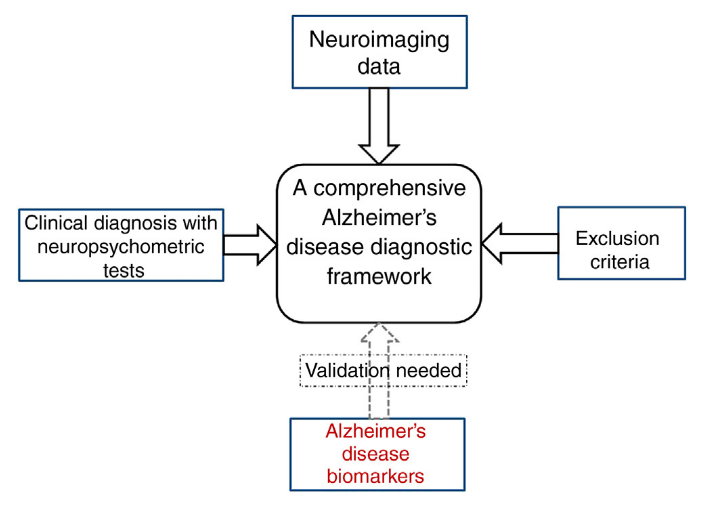
\includegraphics[scale=0.35]{assets/images/alzhemier_diagnosis_scheme.png}
\caption{\textbf{Komplexný rámec pre diagnózu alzheimerovej choroby}. Pozostáva z neuropsychometrických testov, rádiologických snímok (z PET, MRI...), biologických ukazovateľov (napr. úrovne hladín určitých proteínov v krvnej plazme) Alzheimerovej choroby a kritérií vylúćenia iných neurologických chorôb.\cite{khan2016biomarkers}}
\label{fig:alzheimer_diagnosis_scheme}
\end{figure}

\subsection{Biologické ukazovatele}
% angl. biomarkers

Biologické ukazovatele (angl. biomarkers) sú merateľné biologické ukazovatele slú-žiace na detekciu prítomnosti choroby.
% Toto by som najradsej odcitoval, pretoze tato veta je vyplodom precitani asi 5 zdrojov, ale vsade je to opisane velmi z "medical point of view" https://en.wikipedia.org/wiki/Alzheimer%27s_disease_biomarkers
National Insitute of Health definguje biologický ukazovateľ ako indikátor určitého objektívneho merania a hodnotenia biologického procesu, patogénneho procesu alebo farmakologického hodnotenia terapeutickej účinnosti \cite{working2001biomarkers}. Alzheimerova choroba môže byť identifikovaná sledovaním týchto biologických ukazovateľov napríklad v krvnej plazme \cite{khan2016biomarkers} alebo v mozgovomiechovej tekutine (angl. cerebrospinal fluid) (ako úrovne hladín proteínov P-tau and A$\beta$42) \cite{khan2016biomarkers} (angl. cerebrospinal fluid).

\subsection{Obrazové a rádiologické ukazovatele}
% angl. image and radiogological markers, alebo neuroimaging
% ako prelozim neuroimaging???

Identifikovanie Alzheimerovej choroby je v súčastnosti možné aj z rádiologických snímkov. Tvorba rádiologických snímkov je v súčasnosti možná pomocou techník akými sú počítačová tomografia s jednou fotónovou emisiou (angl. single-photon emission computed tomography - SPECT),
pozitrónová emisná tomografia (angl. positron emission tomography PET), počítačová tomografia (angl. computed tomography - CT), magnetická rezonancia (magnetic resonance imaging - MRI) a magnetická rezonančná spektroskopia (angl. magnetic resonance spectroscopy - MRS) \cite{khan2016biomarkers}.

Snímky z magnetickej rezonancie (MRI) dokážu zachytiť odumieranie tkaniva (na základe biologických procesov), ktoré sa odohráva v rôznych častiach mozgu \cite{khan2016biomarkers}. Príklad takého snímku sa nachádza na obrázku \ref{fig:mri_brain_antrophy}.

% TODO: Spomenut: MRI (structural), FMRI, MRS?

\begin{figure}[h!]
    \centering
    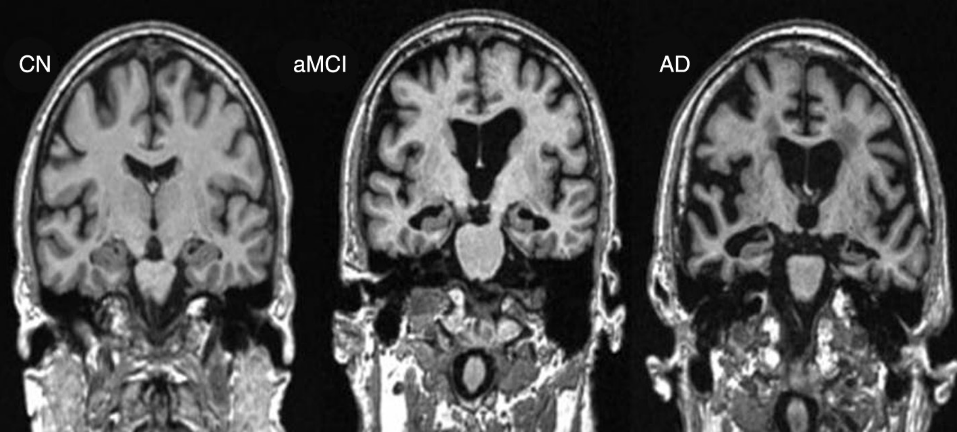
\includegraphics[scale=0.3]{assets/images/mri_brain_antrophy.png}
    \caption{\textbf{Typické odumieranie mozgového tkaniva zachytené magnetickou rezonanciou.} Obrázok zľava, označený ako CN (angl. cognitive normal), reprezentuje kognitívne normálneho jedinca. Obrázok v strede, označený ako aMCI (angl. amnestic mild cognitive impairment) reprezentuje jedinca s miernym kognitívnym poškodením - na obrázku je zreteľný úbytok mozgového tkaniva (šedá farba) najmä v strede mozgu (ale aj na jeho okrajoch) oproti kognitívne normálnemu jedincovi. Posledný obrázok označený ako AD (angl. Alzheimer’s disease) reprezentuje jedinca s Alzheimerovou chorobou - na obrázku je zreteľný značný úbudok mozgového tkaniva. \cite{khan2016biomarkers}
    } 
    \label{fig:mri_brain_antrophy}
\end{figure}

Snímky z pozitrónovej emisnej tomografie (PET) dokážu zachytiť pokles mozgovej aktivity, ktorá je u pacientov s Alzheimerovou chorobou nižšia. Mozgová aktivita odráža úroveň metabolizmu glukózy v mozgu. Na miestach v mozgu, ktoré sú touto chorobou postihnuté, je úroveň metabolizmu glukózy nižšia. Tento jav je znázornený na obrázku \ref{fig:pet}.

\begin{figure}[h!]
    \centering
    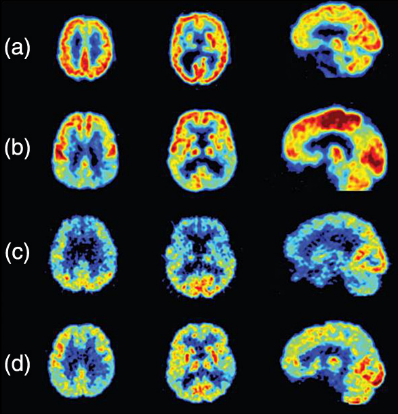
\includegraphics[scale=0.5]{assets/images/pet.png}
    \caption{\textbf{Snímky normálneho mozgu a mozgu postihnutého Alzheimerovou chorobou z pozitrónovej emisnej tomografie (PET).} \cite{khan2016biomarkers}
    Na obrázkoch je viditeľná úroveň metabolizmu glukózy, u pacientov s Alzheimerovou chorobou je táto úroveň nižšia (žltá a modrá farba na obrázkoch).
    (a) Mozog kognitívne zdravého jedinca - vyznačuje sa vyššou mozgovou aktivitou.
    (b) Mozog vyznačujúci symptómy Alzheimerovej choroby - je vidieť nižšiu aktivitu v niektorých častiach mozgu oproti kognitívne zdravému jedincovi.
    (c) Mozog postihnutý frontotemporálnou demenciou (angl. frontotemporal dementia), tiež sa vyznačuje nižšou mozgovou aktivitou.
    (d) Mozog postihnutý Alzheimerovou chorobou.
    } 
    \label{fig:pet}
\end{figure}

% Príklad snímku z MRI je zobrazený na obrázku \ref{fig:mri}.

% \begin{figure}[h!]
% \centering
% 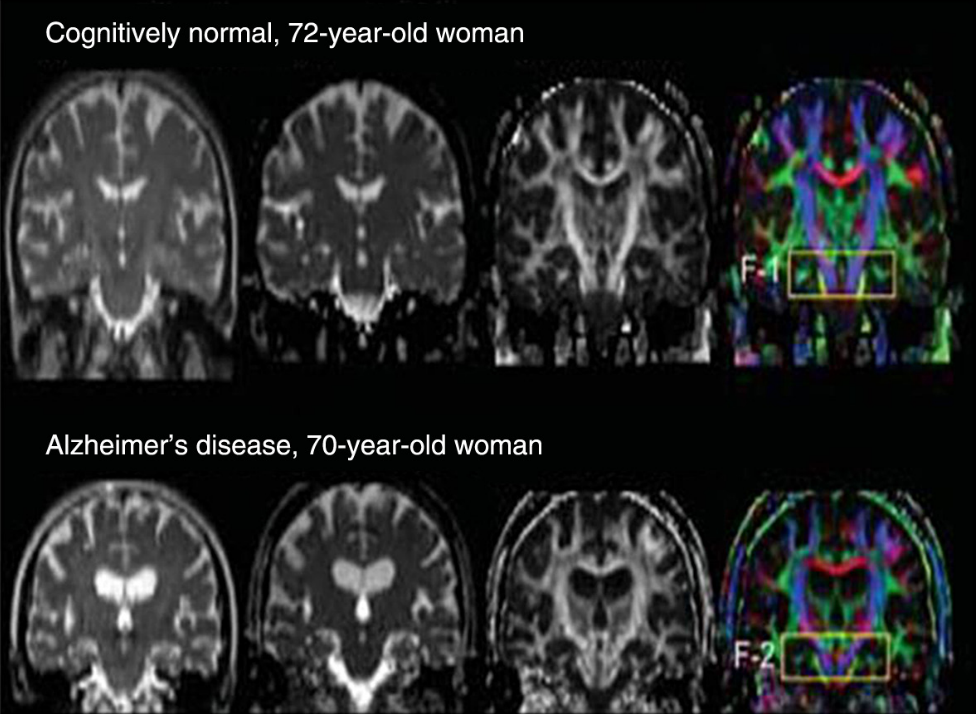
\includegraphics[scale=0.6]{assets/images/mri.png}
% \caption{Zobrazenie difúzneho tenzora (DTI) mozgu pacienta s Alzheimerovou chorobou v porovnaní s kognitívne normálnym jedincom. \cite{khan2016biomarkers} % Obrázok je prevzatý z "Biomarkers in Alzheimer’s Disease", \citeauthor{khan2016biomarkers} \citeyear{khan2016biomarkers}
% }
% \label{fig:mri}
% \end{figure}

\section{Neurónové siete}

Neurónové siete patria medzi obľúbené techniky strojového učenia. Špeciálnou kategóriou sú hlboké neurónové siete (často označované skratkou DNN od angl. deep neural network), ktoré sa oproti obyčajným neurónovým sieťam odlišujú počtom vrstiev. Hlbokým neurónovým sieťam sa doteraz podarilo dosiahnuť v mnohých úlohách výnimočné výsledky, v ktorých častokrát už dokázali poraziť človeka. V našej oblasti obrazových rádiologických dát sa používajú najmä konvolučné neurónové siete.

\citeauthor*{haykin2009neural} \cite{haykin2009neural} definujú neurónovú sieť nasledovne: 
\begin{quote}Neurónová sieť je veľký paralelný distribuovaný procesor tvorený jednoduchými procesorovými jednotkami, ktorý má prirodzený sklon ukladať poznatky a sprístupňovať ich na použitie. Ľudskému mozgu sa podobá v dvoch aspektoch: 
    \begin{enumerate}
        \item Neurónová sieť získava vedomosti zo svojho prostredia prostredníctvom procesu učenia.
        \item Na uchovanie získaných poznatkov sa používajú prepojenia medzi jednotlivými neurónami.
    \end{enumerate}
\end{quote}
Neurónové siete sú teda inšpirované fungovaním mozgu človeka, keďže napodobňujú jeho fungovanie.

\subsection{Neurón} 

Neurón (Obr. \ref{fig:neuron}) je základnou stavebnou jednotkou neurónových sietí. Matematicky sa dá zapísať ako \cite{haykin2009neural}:

\begin{equation}
    y_k = \varphi(b_k + \sum_{j=1}^{m} w_{kj}\cdot x_j)
    \label{eq:neuron}
\end{equation}

Kde:
\begin{itemize}
    \item $x_1, x_2, ... x_m$ sú vstupné signály
    \item $w_{k1}, x_{k2}, ... x_{km}$ sú váhy neurónu $k$
    \item $b_k$ je sklon neurónu $k$
    \item $\varphi(...)$ je aktivačná funkcia
    \item $y_k$ je výsupný signál neurónu $k$
\end{itemize}

Parametrami, ktoré sa počas trénovania neurónovej siete menia sú váhy $w_{kj}$ a sklon $b_{k}$, tieto parametre sú takzvané trénovateľné parametre. Tieto parametre sa upravujú pri spätnej propagácii (angl. backpropagation), kedy sa minimalizuje chybová funkcia (angl. loss function).

V neurónových sieťach s viac vrstvami sa stávajú výstupné signály $y$ neurónov jednej vrstvy vstupom $x$ do ďaľšej.

Aktivačná funkcia zabezpečuje nelinearitu neurónu, medzi najpoužívanejšie aktivačné funkcie patria Sigmoid ($S(x) = \frac{1}{1 + e^x}$), Tanh alebo ReLU ($ReLU(x) = max(0, x)$). Jednotlivé neuróny si môžeme predstaviť ako nelineárne funkcie, ktorých spojením do viac vrstiev dokážu skladať ešte zložitejšie a komplexnejšie funkcie.

\begin{figure}[h!]
    \centering
    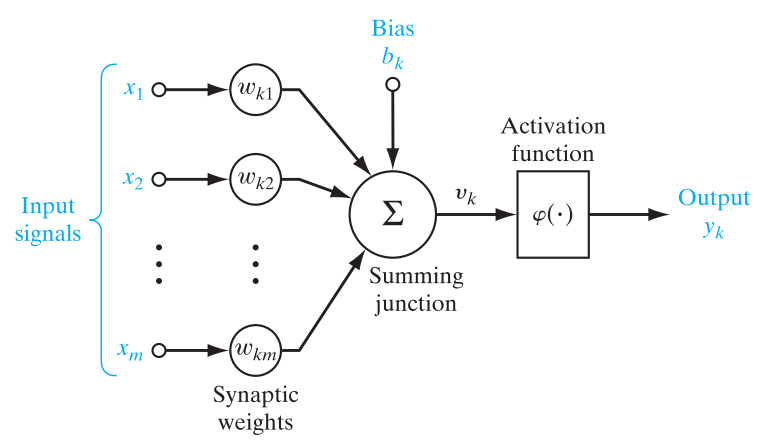
\includegraphics[scale=1]{assets/images/neuron.png}
    \caption{\textbf{Model neurónu.} \cite{haykin2009neural} Neurón sa skladá zo vstupných signálov a váh, ktoré sú na tieto signály aplikované, sklon ($b_k$ - angl. bias) a aktivačnej funkcie, ktorá zapezpečuje nelinearitu. Vzorec \ref{eq:neuron} matematicky popisuje správanie neurónu.} 
    \label{fig:neuron}
\end{figure}

\subsection{Dopredné neurónové siete}

Dopredné neurónové siete (Obr. \ref{fig:ff_nn}) sú jednou z mnoha architektúr neurónových sietí. V dopredných neurónových sieťach výstupný signál z jednej vrsvy nemôže byť vstupným signálom do jej predošlej vrstvy. Signál je prenášaný iba v jednom smere -- dopredu. Dopredné neurónové siete sa môžu skladať z viacerých vrstiev. Základom je vstupná a výstupná vrstva a ľubovolný počet skrytých vrstiev. Ich počet nie je limitovaný, avšak v hlbokých neurónových sieťach (tj. sieťach s veľkým početom skrytých vrstiev) môže nastať problém miznúceho gradientu.

\begin{figure}[h!]
    \centering
    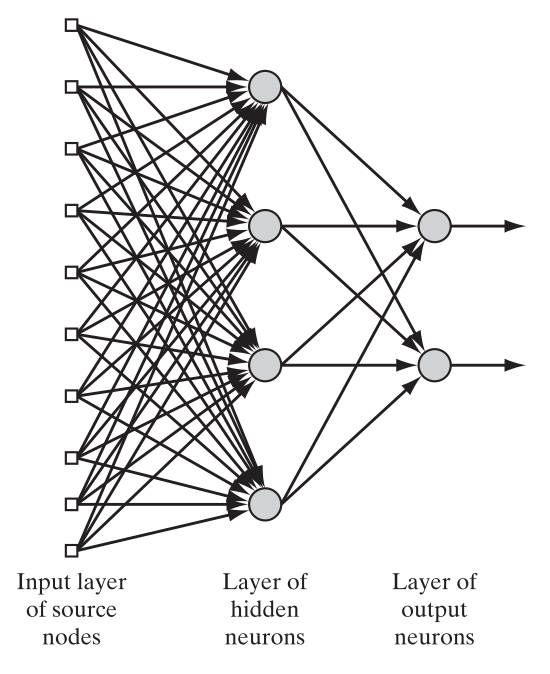
\includegraphics[width=8cm]{assets/images/ff_nn.png}
    \caption{\textbf{Model doprednej neurónovej siete.} \cite{haykin2009neural} Dopredné neurónové siete sa skladajú zo vstupnej vrstvy, skrytých vrstiev a výstupnej vrstvy. Keď hovoríme o počte vrstiev vstupnú vrstvu nepočítame. Neurónová sieť na obrázku má teda dve vrstvy.}
    \label{fig:ff_nn}
\end{figure}

\subsection{Konvolučné neurónové siete}

Konvolučné neurónové siete sa používajú prevažne v doméne obrazových dát. Tieto siete majú schopnosť naučiť sa rozpoznávať špecifické štruktúry/tvary z obrázka. Toto dokážu pomocou takzvaných konvolučných filtrov, ktoré sa v nižších vrstvách naučia rozoznávať jednoduchšie tvary, akými sú napríklad obrysy alebo hrany (Obr. \ref{fig:cnn}). V tých vyšších vrstvách sú to zložitejšie štruktúry akými môžu byť celé objekty v závislosti od typu úlohy na ktorú boli trénované. Ak bola neurónová sieť trénovaná napríklad na klasifikáciu zvierat, môže tým objektom byť pes alebo morča, v prípade ak je úlohou neurónovej siete detekcia Alzheimerovej choroby možu týmito objektami byť niektoré väčšie časti mozgu (napr. hippocampus).

\begin{figure}[h!]
    \centering
    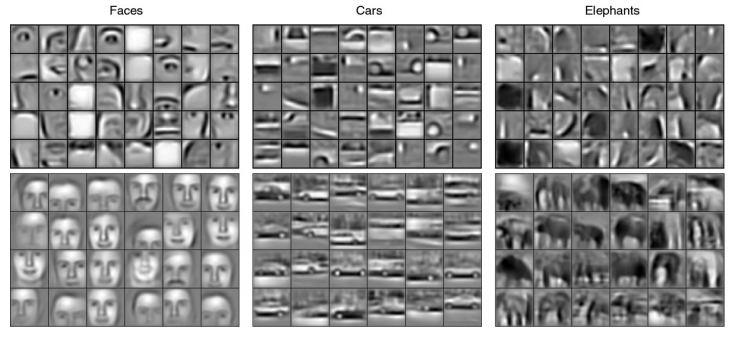
\includegraphics[scale=0.5]{assets/images/cnn.png}
    \caption{
        Vizualizácia druhej (hore) a tretej vrstvy (dole) konvolučných neurónových sietí naučených na špecifické kategórie objektov (tváre, autá a slony). \cite{Lee_Grosse_Ranganath_Ng} Nižšie vrstvy rozoznávajú jednoduchšie štruktúry zatiaľ čo vyššie už dokážu rozonávať aj tie zložitejšie.
    }
    \label{fig:cnn}
\end{figure}

Základnými stavebnými blokmi konvolučných neurónových sietí sú konvolučné vrstvy (angl. convolutional layers) a združovacie vrstvy (angl. pooling layers).

\paragraph{Konvolučné vrstvy}

Pomocou konvolučných vrstiev sa neurónová sieť učí extrahovať črty z obrázka \cite{haykin2009neural}. Konvolúcia prebieha tak, že tzv. jadro (angl. kernel) sa posúva po tzv. mape vlastností (angl. feature map) a matematickými operáciami z pôvodnej mapy vlastností a svojich parametrov vytvára novú mapu vlastností. Tieto parametre sú trénovateľné, čo umožňuje sa každému jadru naučiť urćitú črtu - napr. hranu. Konvolučná vrstva tiež dokáže znižovať kompexitu modelu (a teda aj počet jeho parametrov) jej hyper parametrami (angl: stride, padding, depth).

\paragraph{Združovacie vrstvy}

Cieľom združovacích vrstiev je postupne znižovať dimenzionalitu dát, tým znižovať počet počet parametrov modelu, a teda aj jeho komplexitu \cite{o2015introduction}. Najčastejšie sa používajú vrstvy združujúce maximom (angl. max-pooling), ale existujú aj vrsvy združujúce priemerom či súčtom.

\begin{figure}[h!]
    \centering
    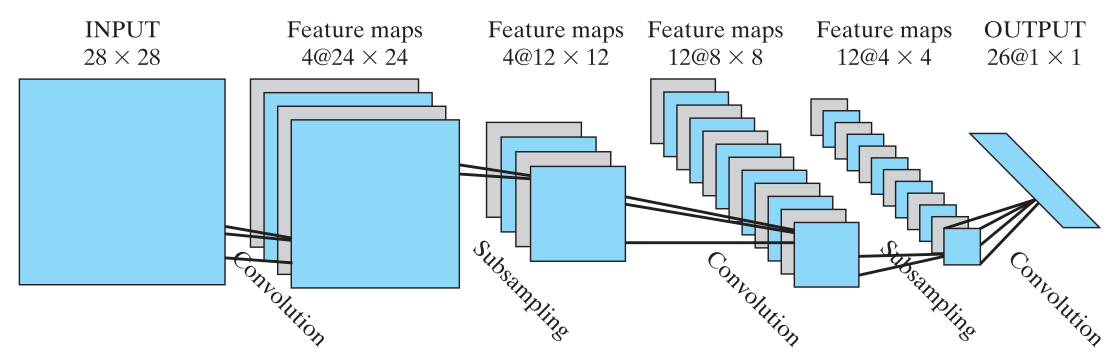
\includegraphics[width=12cm]{assets/images/conv_net_architecture.png}
    \caption{\textbf{Príklad architektúry konvolučnej neurónovej siete. \cite{haykin2009neural}} V tejto achitektúre neurónovej siete sa používajú tri konvolučné vrstvy (označené ako \textit{convolution}) a dve združovacie vrstvy (označené ako \textit{subsampling}). Môžeme si všimnúť, že konvolučné vrstvy postupne pridávajú mapy vlastností (tiež ozačované ako: angl. ''volumes'') a tiež mierne znižujú ich veľkosť. Združovacie vrstvy zasa výrazne znižujú ich veľkosť (až o polovicu) a tým aj počet parametrov v neurónovej sieti.}
    \label{fig:conv_net_architecture}
\end{figure}

\subsection{Interpretovanie neurónovej siete}

\citeauthor{montavon2018methods} (\citeyear{montavon2018methods}) definujú interpretovanie ako mapovanie abstraktného konceptu (napríklad predikovanej triedy) do domény, ktorej človek dokáže porozumieť. Ako príklad domény, ktorá je interpretovateľná uvádzajú obrázky (pole pixelov) alebo text (sekvencia slov) \cite{montavon2018methods}. Medzi domény, ktoré nie sú interpretovateľné zaraďujú napríklad latentné vektorové reprezentácie slov (angl. word embeddings) alebo iné abstraktné vektorové reprezentácie \cite{montavon2018methods}.
Na rozdiel od vstupných dát do neurónovej siete, ktoré sú zvyčajne interpretovatelné, neuróny na výstupnej vrstve a v skrytých vrstvách sú abstraktné a vyžadujú dodatočné úsilie na ich interpretovanie. Jedným zo spôsobov interpretovania týchto neurónov je maximalizácia aktivácie (angl. activation maximization).

\paragraph{Maximalizácia aktivácie (angl. Activation maximization)}
Maximalizácia aktivácie je metóda na nájdenie takého vstupného prototypu, ktorý vyprodukuje najväčšiu mieru aktivácie pre zvolený neurón (zvyčajne je to neurón hľadanej triedy na najvyššej vrstvy). 
% Takýto vstupný prototyp je nájdený optimalizovaním nasledovnej funkcie pomocou poklesu gradientu (angl. gradient descent).
Takýto vstupný prototyp je nájdený tak, že neurónovej sieti je daný na vstup neutrálny obrázok, ktorý v danej doméne nereprezentuje žiadnu triedu (zvyčajne sa jedná o šedý obrázok) a je optimalizovaná funkcia maximalizácie aktivácie pomocou poklesu gradientu \cite{montavon2018methods} (angl. gradient descent). Pri aplikovaní tejto metódy na obrazové dáta výsledné prototypy vyzerajú tak ako na obrázku \ref{fig:activation_maximization}.

\begin{figure}[h!]
\centering
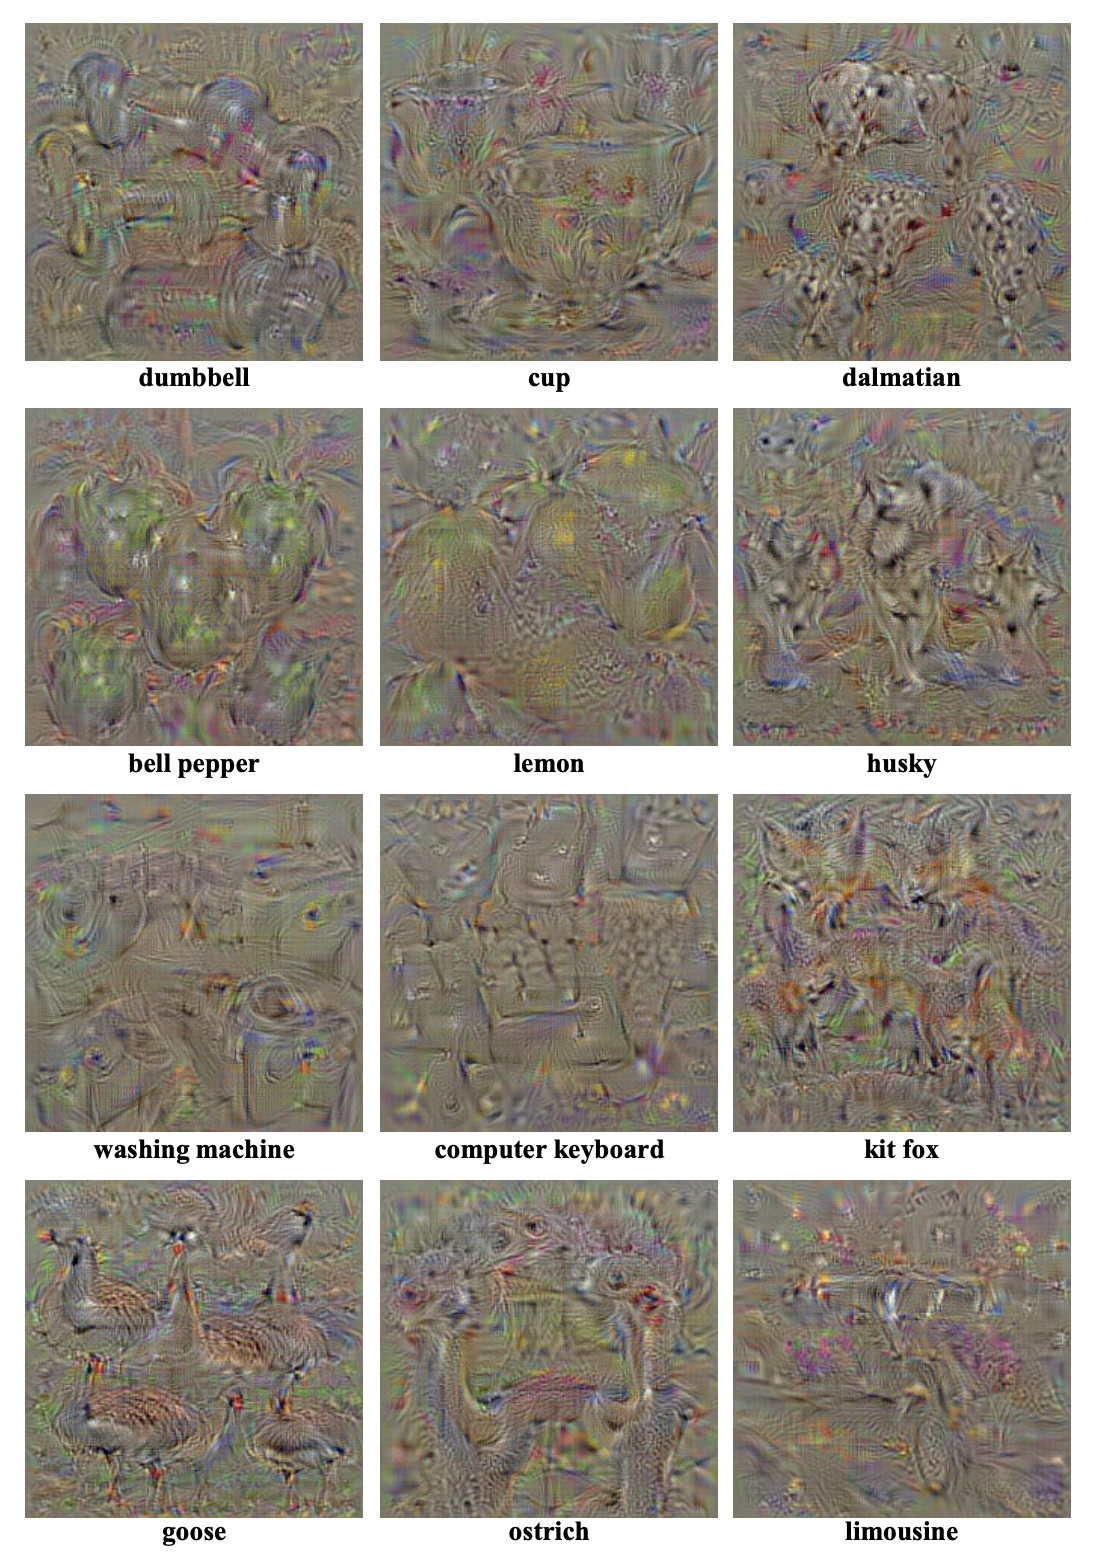
\includegraphics[scale=0.6]{assets/images/activation_maximization.png}
\caption{\textbf{Maximalizácia aktivácie aplikovaná na obrazové dáta. \cite{simonyan2013deep}} Výsledné vzorové prototypy pre jednotlivé triedy nevyzerajú prirodzene, sú prevažne šedé s farebnými črtami objektov. Tieto vzorové prototypy nereprezentujú príklady vstupov ''z reálneho sveta'' ale ideálne vstupy pre jednotlivé triedy. Takéto vstupy nerónová sieť bežne nedostane.
}
\label{fig:activation_maximization}
\end{figure}

\paragraph{Maximalizácia aktivácie s expertom}
Na získanie realistickejších prototypov (prototypov, ktoré sa viac podobajú vstupným dátam) $l_2$-regularizácia (používaná v maximalizácii aktivácie) je nahradená takzvaným ``expertom``, ktorý sa snaží naučiť distribúciu hľadanej triedy \cite{montavon2018methods}. Oproti $l_2$-regularizácii, ktorá hľadá vstup maximalizujúci pravdepodobnosť triedy, expert hľadá taký vstup, ktorý je najpravdepodobnejší pre zvolenú triedu. Ako ``expert`` môže byť použitý napríklad Gaussian RBM (angl. Restricted Boltzmann machine) \cite{montavon2018methods}.
% TODO: niesom si isty, opytat sa "naučiť distribúciu hľadanej triedy", a ta posledna veta ci citovat prehladovy clanok alebo clanok z prehladoveho clanku ktory som ani necital

% AM in code space, doplnit? Tam sa pouzivaju tie GAN...
% TODO: AM in code space
% k tomu je velmi prijemny obrazok tuto http://iphome.hhi.de/samek/pdf/DTUSummerSchool2017_1.pdf

\subsection{Vysvetľovanie predikcie neurónovej siete}

\citeauthor{montavon2018methods} (\citeyear{montavon2018methods}) definujú vysvetľovanie ako kolekciu vlastností dát, ktoré sú z interpretovateľnej domény, ktoré prispeli k výslednému rozhodnutiu (napr. zaradenie do určitej triedy - klasifikácia) pre určité pozorovanie \cite{montavon2018methods}. Rozdiel oproti interpretovaniu teda je, že pri interpretovaní hľadáme vzorový prototyp (vzorové pozorovanie) pre zvolenú triedu, zatiaľ čo pri vysvetľovaní sa snažíme zistiť prečo, a teda ktoré z vlastností vstupu najviac prispeli (tj. sú najviac relevantné) k výslednej predikcii neurónovej siete (napr. zaradenie pozorovania do určitej triedy). 

Niektoré metódy vysvetľovania fungujú na základe zakrývania častí obrázka a sledovaním zmeny predikcie predikovanej triedy -- perturbačné metódy, iné zasa na základe spätného šírenia (angl. backpropagation) -- napr. LRP, analýza senzitivity.

Každá z metód má svoje výhody a nevýhody, napríklad výhodou perturbačných metód je, že môžu byť použité na akýkoľvek model, keďže jediné čo potrebujú je výstup (predikciu) z modelu. Ich nevýhodou však je, že sú pomalé. Niektoré z metód vysvetľovania bližšie opíšeme v tejto sekcii.

\subsubsection{Analýza senzitivity}

Analýza senzitivity slúži na vysvetľovanie predikcie neurónovej siete. Táto metóda identifikuje, ktoré z vlastností vstupného pozorovania najviac prispievajú, či už pre alebo proti, výslednej predikcii. Najviac dôležité sú také vlastnosti, ktorých zmenou sa najvýraznejšie zmení výsledná predikcia. Na takéto vlastnosti je výsledná predikcia najviac citlivá \cite{montavon2018methods}.

Výsledok analýzy senzitivity znázornený v tepelnej mape (angl. heatmap) je zobrazený na obrázku \ref{fig:sensitivity_analysis}. Analýza senzitivity zachytáva teda vlastnosti vstupného pozorovania, ktoré k výslednej predikcii prispievajú pozitívne aj negatívne (napr. zmenením určitej vlastnosti vstupu sa výrazne zníži zaradenie do danej triedy). Na výslednej tepelnej mape vlastnosti, ktoré k výslednej predikcii prispievajú pozitívne, a vlastnosti, ktoré k výslednej predikcii prispievajú negatívne (proti), nevieme rozlíšiť. Vieme len, že zmenením danej vlastnosti výrazne ovplyvníme predikciu.

\begin{figure}[h!]
\centering
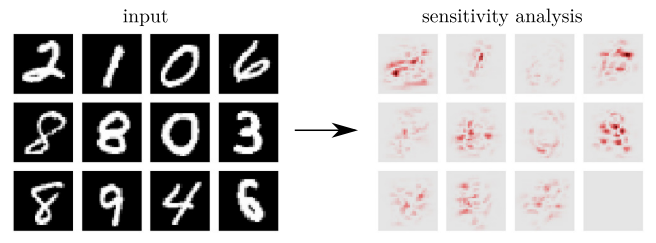
\includegraphics[scale=0.5]{assets/images/sensitivity_analysis.png}
\caption{\textbf{Analýza senzitivity aplikovaná na konvolučnú neurónovú sieť trénovanú na dátovej sade MNIST. \cite{montavon2018methods}} Červenou farbou sú zobrazené miesta ktoré najviac prispievajú, či už pre alebo proti, výslednej predikcii. Čím je červená farba výraznejšia, tým viac je výsledok senzitívny na zmenu daného pixela.}
\label{fig:sensitivity_analysis}
\end{figure}

\subsubsection{LRP (angl. layer-wiser relevance propagation)}

Metóda vrstvami propagovanej relevancie, ďalej len LRP (angl. layer-wise relevance propagation), sa od analýzy senzitivity odlišuje tým, že vo výslednej tepelnej mape dokáže odlíšiť vlastnosti, ktoré prispeli pozitívne alebo negatívne k výslednej predikcii (v zázislosti od použitých parametrov $\alpha$ a $\beta$).

Táto technika funguje tak, že vstupný obrázok dopredným šírením ''prejde'' neurónovou sieťou, pričom sú zozbierané aktivácie neurónov v jednotlivých vrstvách. Následne je neurónovou sieťou spätným šírením propagované skóre z výstupu neurónovej siete v podobe relevancie až k vstupnému obrázku. 

Nasledovné vzorce \ref{eq:lrp_1}, \ref{eq:lrp_2}, \ref{eq:lrp_3} \cite{montavon2018methods} vyjadrujú spôsob výpočtu propagovanej relevancie medzi vrstvami. $j$ a $k$ sú jednotlivé vrstvy, pričom $k$ je vrstva, z ktorej je relevancia $R$ propagovaná. Parametre $\alpha$ a $\beta$ upravujú, koľko pozitívnej ($\alpha$) alebo negatívnej ($\beta$) relevancie je vytvorenej počas fázy spätného šírenia relevancie. Pri ich nastavovaní musí platiť, že $\alpha - \beta = 1$ a zároveň $\beta \geq 0$. Súčet pozitívnej a negatívnej relevancie je však medzi vrstvami vždy rovnaký \cite{montavon2018methods}, výsledok použitia rôznych hodnôt $\alpha$ a $\beta$ je znázornený na obrázku \ref{fig:lrp}. $R_{j\leftarrow k}^{+}$ (Obr. \ref{eq:lrp_1}) a $R_{j\leftarrow k}^{-}$ (Obr. \ref{eq:lrp_3}) vyjadrujú množstvo pozitívnej ($+$), resp. negatívnej ($-$) relevancie propagovanej z vrstvy $k$ do vrstvy $j$. $a_j$ je aktivácia neurónu, na ktorý je propagovaná relevancia.

% Option 1
% \begin{equation}
%     R_{j}=\sum_{k}^{}\frac{a_j w_{j k}^+}{\sum_{j}^{} a_j w_{j k}^+}\alpha R_k + \sum_{k}^{}\frac{a_j w_{j k}^-}{\sum_{j}^{} a_j w_{j k}^-}\beta R_k
%     \label{eq:lrp}
% \end{equation}

% Option 2
\begin{equation} 
    R_{j\leftarrow k}^{+} = \frac{a_j w_{j k}^+}{\sum_{j}^{} a_j w_{j k}^+}
    \label{eq:lrp_1}
\end{equation}
\begin{equation} 
    R_{j\leftarrow k}^{-} = \frac{a_j w_{j k}^-}{\sum_{j}^{} a_j w_{j k}^-}
    \label{eq:lrp_2}
\end{equation}
\begin{equation} 
    R_{j}=\sum_{k}^{} \left ( \alpha R_{j\leftarrow k}^{+} - \beta R_{j\leftarrow k}^{-} \right ) R_k
    \label{eq:lrp_3}
\end{equation}

\begin{figure}[h!]
\centering
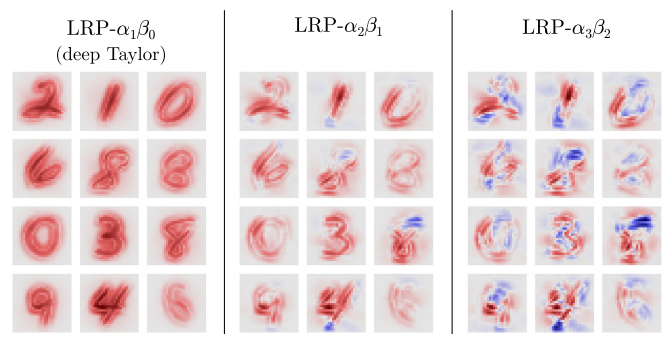
\includegraphics[scale=0.5]{assets/images/lrp.png}
\caption{\textbf{Výsledné vysvetlenie (v podobe tepelnej mapy) vytvorené použitím LRP s rôznymi hodnotami $\alpha$ a $\beta$ na dátovej sade MNIST. \cite{montavon2018methods}} Pozitívna relevancia je zobrazená červenou farbou \cite{montavon2018methods}. Negatívna relevancia je zobrazená modrou farbou \cite{montavon2018methods}. V prípade, že použijeme $\alpha = 1$ a $\beta = 0$ strácame informáciu o tom, ktoré pixely negatívne (tj. sú proti výslednej predikcii) prispeli k výslednej predikcii (a opačne).}
\label{fig:lrp}
\end{figure}

Výhodou LRP oproti analýze senzitivity je, že vysvetlenie (výsledná tepelná mapa) vytvorené technikou LRP je pre rôzne obrázky vždy rôzne \cite{Muller_Samek_Montavon_Lapuschkin_Arras}. Naopak, pri analýze senzitivity je vysvetlenie vždy rovnaké pokiaľ v architektúre neurónovej siete neboli použité združovacie vrstvy (angl. pooling layers) \cite{Muller_Samek_Montavon_Lapuschkin_Arras}. Ďaľším rozdielom je, že vo výslednom vysvetlení LRP rozlišuje, ktoré vlastnosti pozitívne alebo negatívne prispeli k negatívnej predikcii.

% TODO: vysvetlit dekonvoluciu???

\subsubsection{RISE - Randomized Input Sampling for Explanation \label{sec:rise}}

Túto metódu môžeme zaradiť medzi perturbačné metódy, keďže je tiež založená na zakrývaní jednotlivých častí obrazu a sledovaním zmeny výslednej predikcie modelu. Už z názvu modelu \textit{(Randomized Input Sampling for Explanation)} je zrejmé, že táto metóda využíva náhodu na zakrývanie jednotlivých častí vstupného obrazu. Vstupný obraz je prekrytý náhodou maskou, ktorá je vytvorená nasledovne \cite{petsiuk2018rise}:

\begin{itemize}
    \item Je vytvorená náhodná binárna (tj. iba z bielej a čiernej farby) maska o malej veľkosti (napríklad 8px x 8px).
    \item Táto maska je zväčšená (angl. upsampled) pomocou bilineárnej interpolácie \cite{petsiuk2018rise} (angl. bilinear interpolation) na veľkosť ktorá je mierne väčšia ako veľkosť obrázka s ktorým bude prekrytá (kvôli oreznávaniu). Tým sa zníži jej kvalita a ostré hrany medzi bielymi a čiernymi časťami sa zjemnia. Masky už teda nie sú binárne.
    \item Z masky je náhodne vyrezaná náhodná čast o veľkosť prekrývaného obrázka.
\end{itemize}

% To address these issues we first sample smaller binary masks and then upsample them to
% larger resolution using bilinear interpolation. Bilinear upsampling does not introduce sharp edges in I?Mi as well as results in a smooth importance map S.

Toto sa opakuje $N$ krát. Výsledná tepelná mapa je je vypočítaná ako vážený priemer všetkých vygenerovaných masiek, kde váhy sú skóre (pravdepodobnosť predikovanej triedy) z modelu. Tento proces je zobrazený na obrázku \ref{fig:rise_architecture}.

\begin{figure}[h!]
    \centering
    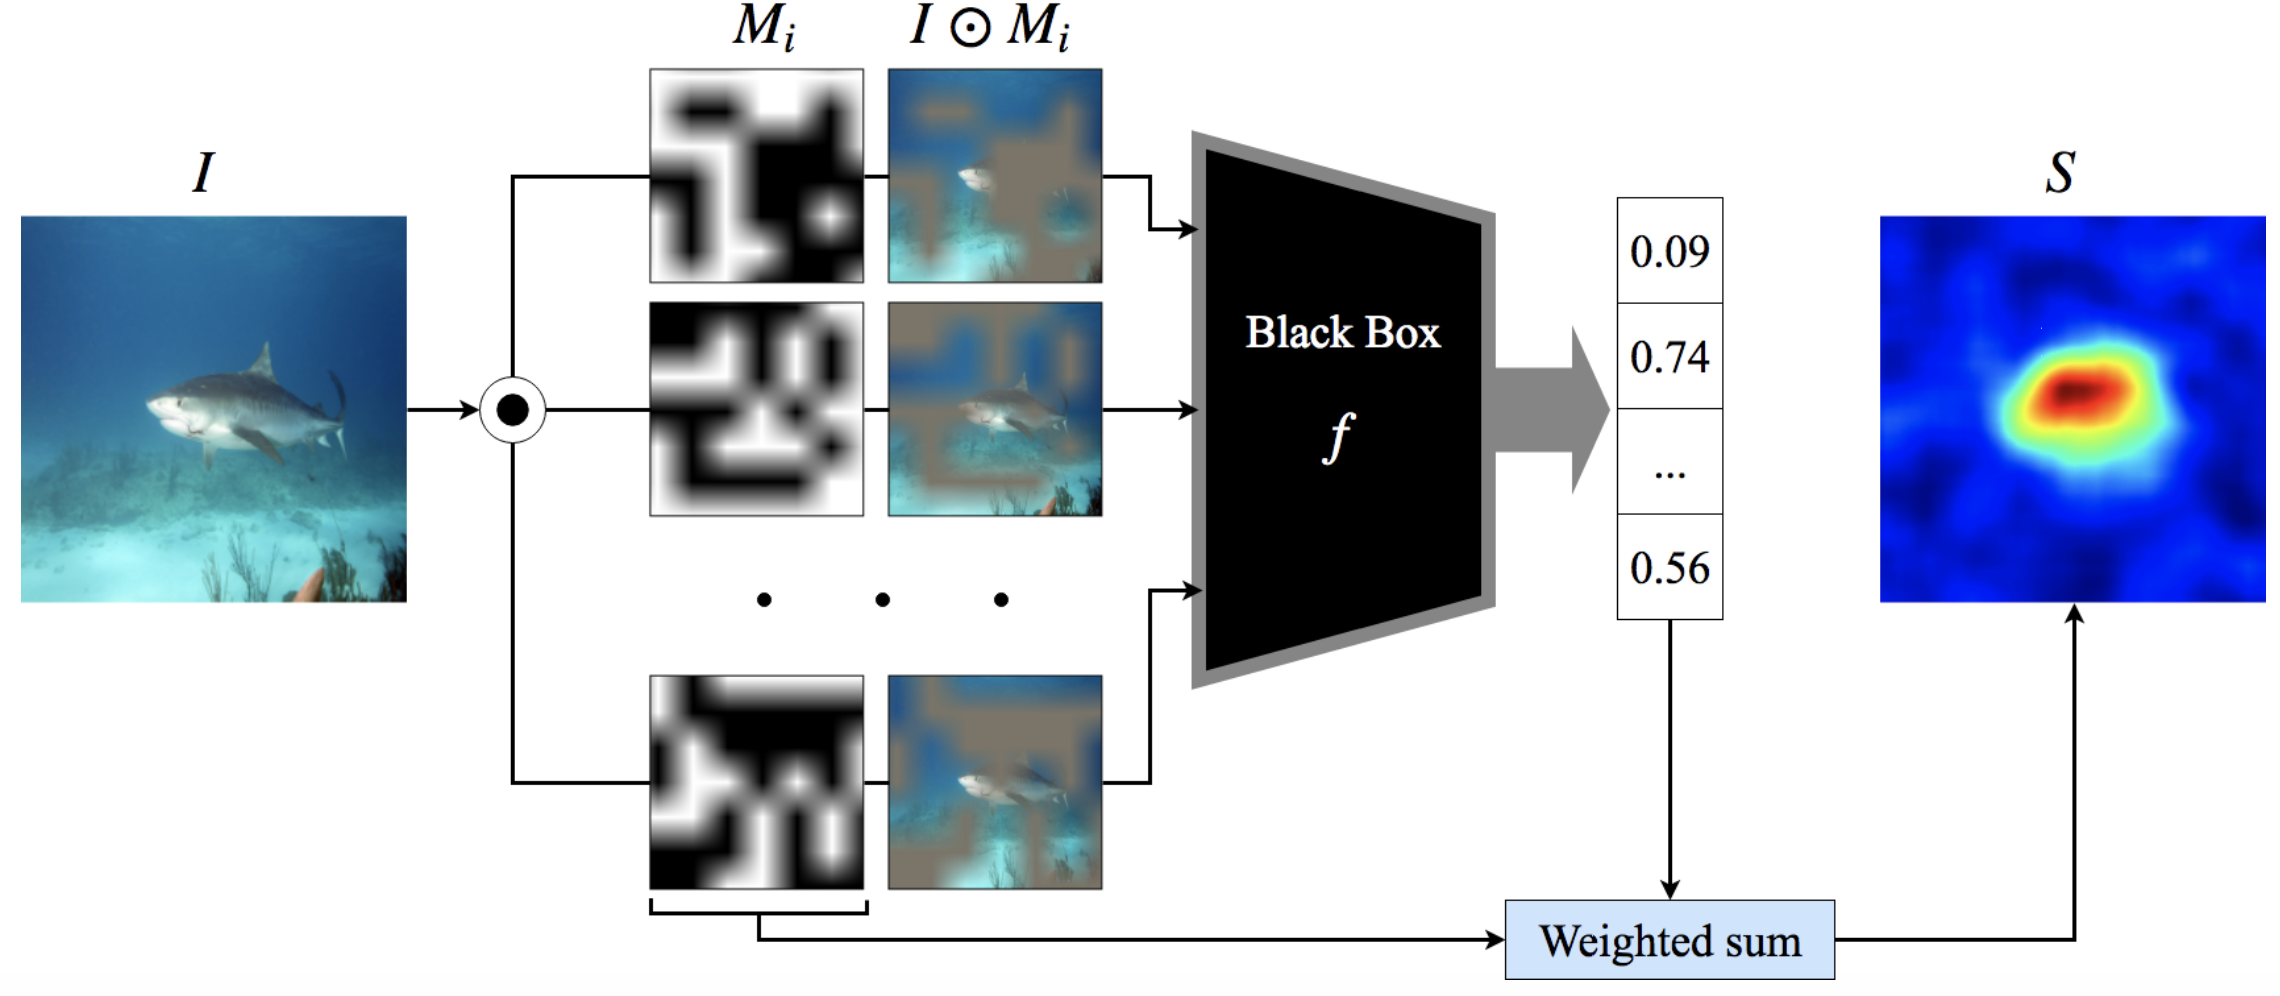
\includegraphics[scale=0.35]{assets/images/rise_architecture.png}
    \caption{Metóda \textit{RISE}. \cite{petsiuk2018rise} Vygenerované masky nahrádzajú vstupný obrázok na, ktorý sú aplikované. Z výstupných predikcii jednotlivých masiek je nakoniec vypočítaná tepelná mapa.}
    \label{fig:rise_architecture}
\end{figure}

Autori porovnali túto metódu s metódami \textit{GradCAM} (\citeauthor*{selvaraju2017grad} \citeyear{selvaraju2017grad}) \cite{selvaraju2017grad} a \textit{LIME} (\citeauthor*{ribeiro2016should} \citeyear{ribeiro2016should}) \cite{ribeiro2016should}. Metóda \textit{RISE} si oproti týmto dvom metódam počínala lepšie (Obr. \ref{fig:rise_results}). Vykonali niekoľko experimentov, v ktorých porovnali architektúry neurónových sietí \textit{ResNet50} (\citeauthor*{he2016deep} \citeyear{he2016deep}) \cite{he2016deep} a \textit{VGG16} (\citeauthor{simonyan2014very} \citeyear{simonyan2014very}) \cite{simonyan2014very} natrénované na dátových sadách PASCAL VOC07 (\citeauthor*{everingham2010pascal} \citeyear{everingham2010pascal}) \cite{everingham2010pascal} a MSCOCO2014 (\citeauthor*{lin2014microsoft} \citeyear{lin2014microsoft}) \cite{lin2014microsoft}. Sledovali metriky \textit{insertion} a \textit{deletion} (Obr. \ref{fig:rise_results}). Metrika \textit{insertion} je vyjadrená ako plocha pod krivkou (AUC) funkcie $y = f(x)$, kde $y$ je istota predikcie a $x$ je počet pridaných najdôležijetších pixelov, dôležitosť pixelov je určená metódou vysvetľovania predikcie neurónovej siete a môže byť zobrazené pomocou tepelnej mapy. Metrika \textit{deletion} naopak odoberá najdôležitejšie pixely z obrázka.

Výhodou tejto metódy je, že oproti bežným perturbačným metódam je výrazne rýchlejšia.

\begin{figure}[h!]
    \centering
    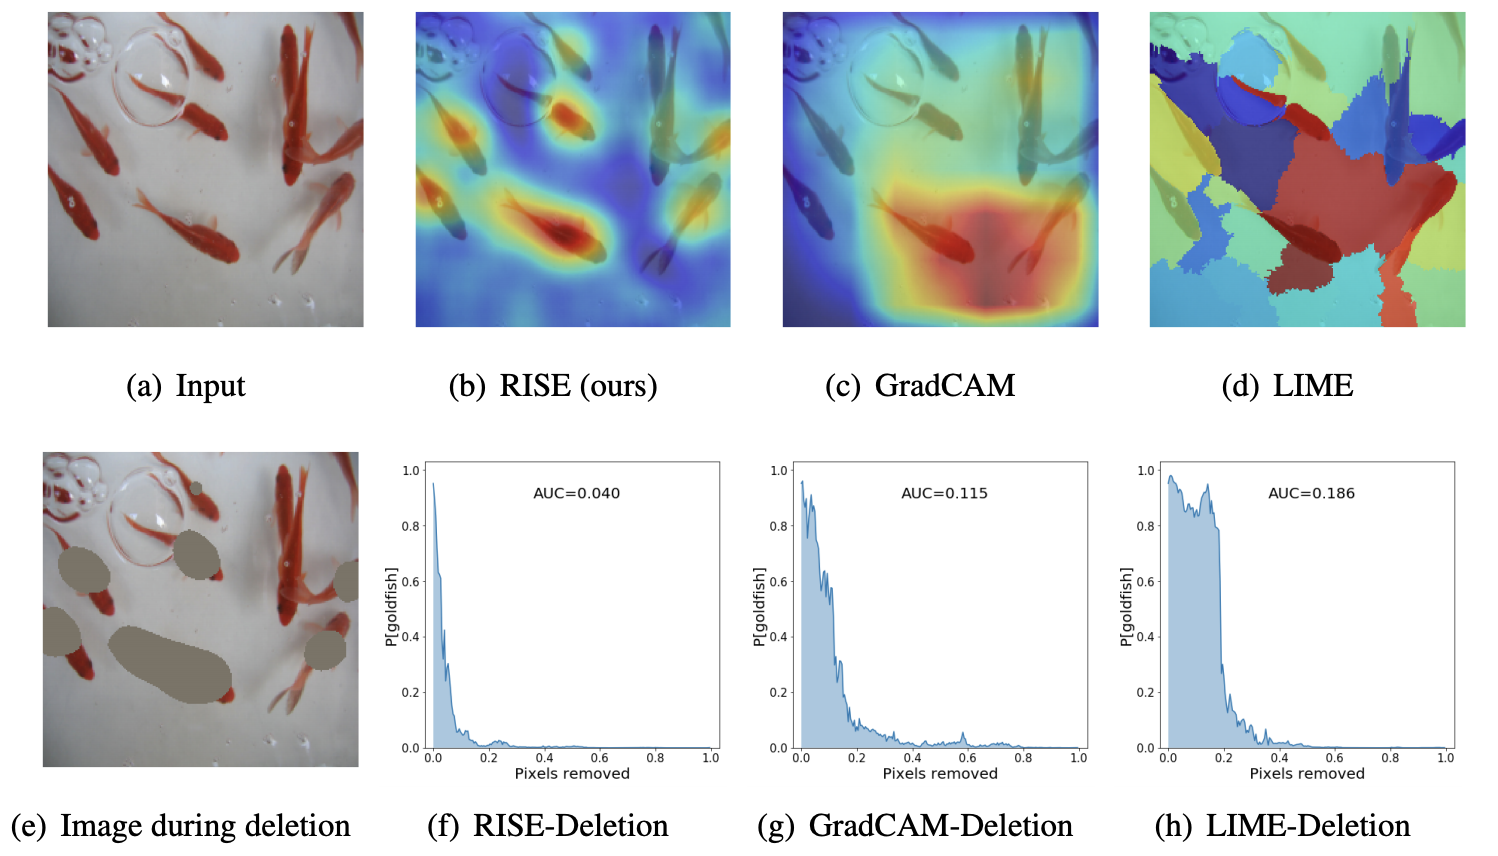
\includegraphics[scale=0.5]{assets/images/rise_results.png}
    \caption{Porovnanie metódy \textit{RISE} s \textit{GradCAM} alebo \textit{LIME}. \cite{petsiuk2018rise} V prvom riadku sú tepelné mapy jednotlivých metód pre vstup. V druhom riadku je znázornená porovnávaná metrika \textit{deletion}. Táto metrika sleduje vzťah medzi odobratím najdôležijetších pixelov a výslednou predikciou modelu. Je vyčíslená pomocou výpočtu plochy pod krivkou (AUC). Na grafoch si môžeme všimnúť, že metóda \textit{RISE} potrebuje odobrať menej pixelov na to aby klesla pravdepodobnosť predikovanej triedy. To znamená, že tepelná mapa (metódy \textit{RISE} oproti ostatným metódam) lepšie zaznamenáva dôležité pixely pre predikovanú triedu.}
    \label{fig:rise_results}
\end{figure}

\section{Využitie neurónových sietí pri odhaľovaní Alzheimerovej choroby \label{sec:nn_ad_prediction}}

Neurónovým sieťam sa doposiaľ podarilo dosiahnuť veľmi dobré výsledky pri odhaľovaní Alzhemiemerovej choroby. Medzi state-of-the-art riešenia patrí konvolučná neurónová sieť (Obr. \ref{fig:ad_cnn_architecture}) od \citeauthor*{esmaeilzadeh2018end} s presnosťou \textbf{94.1\%} (a s $F_2$ skóre 0.93) na populárnej dátovej množine s názvom \textit{ADNI-1}. Tento výsledok dosiahli v úlohe klasifikácie iba do CN a AD (bez MCI). Vstupom do tejto neurónovej siete boli snímky z magnetickej rezonancie (MRI) ale aj demografické informácie akými sú napríklad vek alebo pohlavie. Autor avšak nereportuje úspešnosť modelu, ktorý bol natrénovaný iba z obrazových dát, táto úspešnosť by bola pravdepodobne o niečo nižšia.

\begin{figure}[h!]
    \centering
    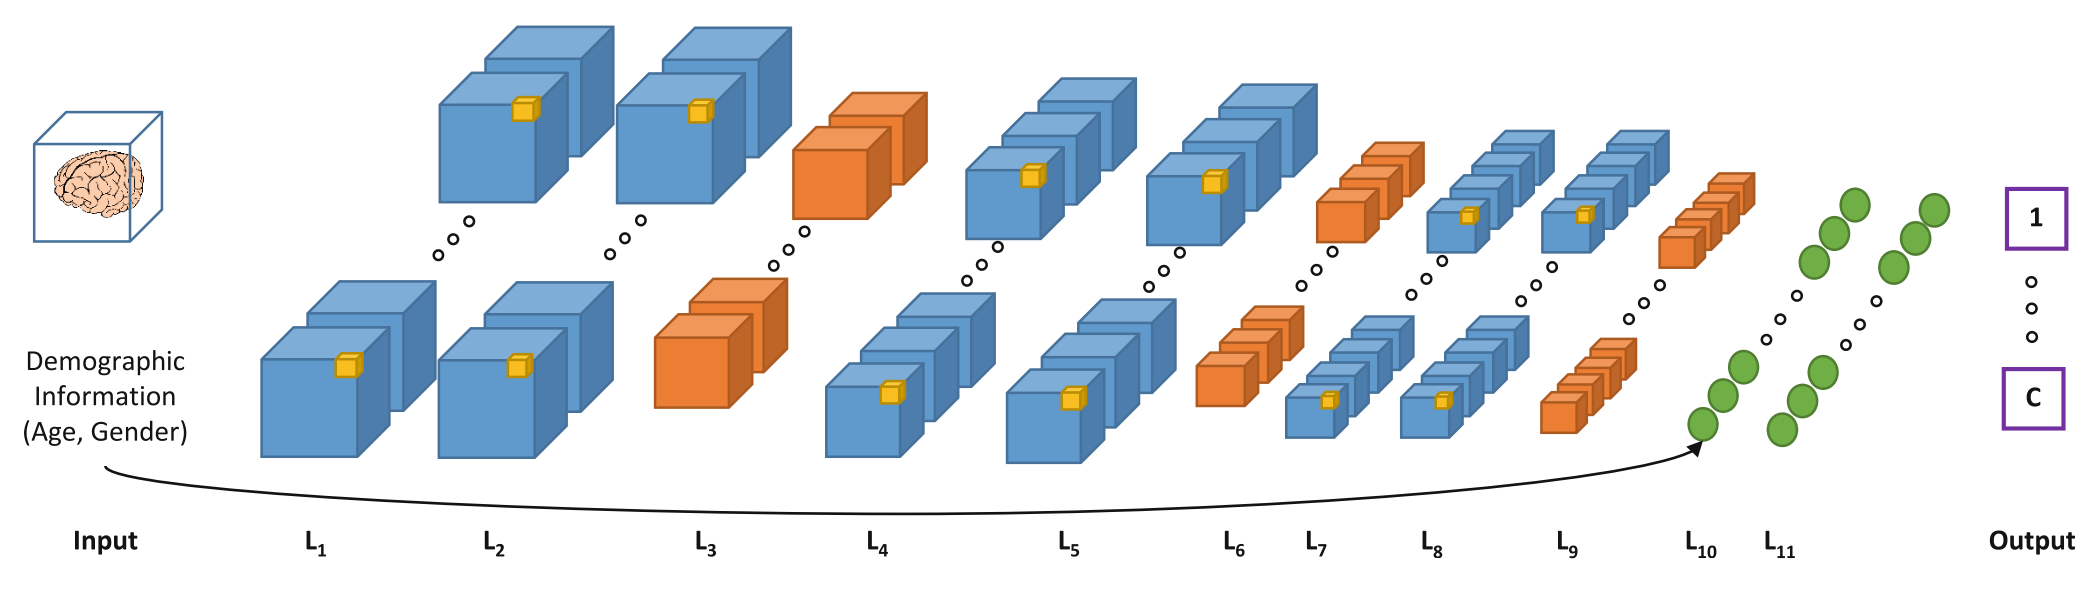
\includegraphics[scale=0.35]{assets/images/ad_cnn_architecture.png}
    \caption{Architektúra konvolučnej neurónovej siete použitej pri detekcii Alzheimerovej choroby. \cite{esmaeilzadeh2018end} Modré kocky sú konvolučné vrstvy, oranžové kocky sú \textit{max-pooling} vrstvy, posledné dve (zelené) vrstvy sú plne prepojené vrstvy. Môžeme si všimnúť, že do posledných dvoch plne prepojených vrstiev okrem obrazových dát vstupujú aj informácie o veku a pohlaví.}
    \label{fig:ad_cnn_architecture}
\end{figure}

V prípade klasifikácie do všetkých troch tried - CN, MCI a AD autori tejto práce dosiahli horšie výsledky oproti binárnej klasifikácii. Ich model dokázal správne zaradiť pacienta s presnosťou \textbf{61.1\%} (a s $F_2$ skóre 0.62) \cite{esmaeilzadeh2018end}. Pri dosiahnutí tohto výsledku použili tzv. učenie s prenosom (angl. transfer learning), ktoré im zlepšilo úspešnosť modelu až o 5.1\% z pôvodných 54\%. Model, z ktorého učili prenosom je už skôršie spomínaný model na binárnu klasifikáciu pacientov s Alzheimerovou chorobou.

Autori experimentovali trénovaním dvoch rôznych modelov, jedného jednoduchšieho a druhého zložitejšieho. Lepší bol jednoduchší model, pretože nebol tak náchylný na pretrénovanie. V týchto modeloch použili dropout, $l_2$ regularizáciu a augmentované dáta (obrázky otočili po osi x). Tieto ''vylepšenia'' pridávali postupne a sledovali rozdiel v úspešnosti modelu, každé jedno z týchto vylepšení výrazne zlepšilo úspešnosť modelu. V kroku predspracovania dát odstránili z obrázkov také časti, ktoré nepredstavovali tkanivo mozgu (napr. lebka) technikou s názvom BET (\citeauthor*{smith2002fast} \citeyear{smith2002fast}) \cite{smith2002fast}, pretože z nich sa Alzheimerova choroba nedá diagnostikovať.

Niektoré práce (\citeauthor*{suk2016deep} \citeyear{suk2016deep}) sa zaoberali dokonca klasifikáciou do štyroch tried: AD, CN, pMCI (angl. progressive MCI - pacienti ktorí pokročili k AD do 18 mesiacov), sMCI (angl. stable MC - pacienti ktorí nepokročili k AD do 18 mesiacov). Táto úloha je samozrejme náročnejšia, najlepší model v tomto prípade dosahoval presnosť 53.72\% \cite{suk2016deep}. V prípade binárnej klasifikácie (AD vs CN) sa autorom podarilo dosiahnuť presnosť až \textbf{95.09}\%, oproti \citeauthor*{esmaeilzadeh2018end} však použili aj rádiologické snímky z PET. Táto práca sa ďalej vyznačuje adaptívnou selekciou čŕt, vďaka ktorej sa autorom podarilo dosiahnuť tak dobré výsledky.


% TODO: translate max-pooling, dropout?

\subsection{Vysvetľovanie rozhodnutí neurónových sietí detegujúcich Alzheimerovu chorobu \label{sec:ad_nn_explanation}}

Existujúce práce sa už zaoberali metódami vysvetľovania rozhodnutí neurónových sietí detekujúcich Alzheimerovu chorobu. \citeauthor{bohle2019layer} \citeyear{bohle2019layer} uviedli možnosti analýzy rozhodnutí za účelom ich vysvetľovania. Konkrétne sa zaoberali metódami vrstvami propagovanej relevancie (LRP) a vedenou spätnou propagáciou (angl. guided backpropagation). Uvádzajú LRP ako metódu na vysvetľovanie invididuálnych rozhodnutí neurónovej siete kde naopak vedenú spätnú propagáciu ako metódu na zistenie oblastí, na ktoré je neurónová sieť senzitívna. Tieto metódy skúmali porovnávaním priemerov tepelných máp (angl. heatmaps) všetkých pozorovaní v predikovaných triedach (2 - AD, HC). Taktiež porovnávali priemerné tepelné mapy pozorovaní podľa spôsobu zaradenia výslednej predikcie (4 - true positive, true negative, false positive, false negative) (Obr. \ref{fig:lrp_alzheimer}). Okrem iného porovnávali mieru relevancie pri metóde LRP v jednotlivých častiach mozgu u pozorovaní s Alzheimerovou chorobou a u pozorovaní bez nej. Možným vylepšením tejto práce je vyskúšanie metódy LRP aj na pacientoch s miernym kognitývnym poškodením (angl. mild-cognitive impairment), nie len na pacientoch s Alzheimerovoch chorobou a zdravých jedincoch.

% TODO: Este nejake prace...

\begin{figure}[h!]
    \centering
    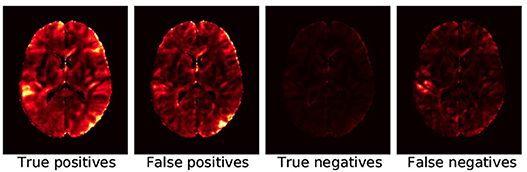
\includegraphics[scale=0.4]{assets/images/lrp_alzheimer.png}
    \caption{
        \textbf{Priemerná relevancia (z metódy LRP - $\beta = 0$) pozorovaní podľa spôsobu zaradenia výslednej predikcie} Najviac relevancie je na miestach so žltou farbou. \cite{bohle2019layer}
    }
    \label{fig:lrp_alzheimer}
\end{figure}

\section{Spracovanie obrazu \label{cap:image_processing}}

Keďže pri diagnostike Alzheimerovej choroby sa pracuje s rádiologickými snímkami, čo sú trojrozmerné obrazové dáta, pri jej detekcii neurónovými sieťami je potrebné tieto dáta spracovať technikami spracovania obrazu.

Metódy spracovania obrazu podľa \citeauthor*{chen2004electrical} \cite{chen2004electrical} rozdeľujeme do nasledovných kategórií:
\begin{itemize}
    \item vylepšovanie obrazu (angl. image enhancement)
    \item rekonštrukcia obrazu (angl. image restoration)
    \item analýza obrazu (angl. image analysis)
    \item kompresia obrazu (angl. image compression)
\end{itemize}

Pri \textbf{vylepšovaní obrazu} je obraz upravovaný predovšetkým heuristickými technikami \cite{chen2004electrical}, môže sa napríkald jednať o upravenie jasu, kontrastu alebo farieb. Cieľom \textbf{rekonštrukcie obrazu} je zrekonštruovať poškodené časti obrazu, napr. pri fotografiách to môžu byť ich vyblednuté časti. Metódy \textbf{analýzy obrazu} umožňujú obraz spracovať tak, že je možné z neho automaticky získať (extrahovať) informácie \cite{chen2004electrical}. Príkladmi analýzy obrazu je segmentácia obrazu, extrakcia hrán alebo analýza textúry. \textbf{Kompresia obrazu} umožňuje zmenšenie veľkosti obrazu znižovaním počtom potrebných bitov na jeho reprezentáciu \cite{chen2004electrical}. Môže sa jednať o zmenšenie rozmerov obrazu, alebo počtu farieb potrebných na jeho reprezentáciu.

V našej doméne budeme pracovať so všetkými týmito technikami. Ako príklad môžem uviesť odstránenie takých častí obrazu, ktoré nepredstavujú mozgové tkanivo (BET - \citeauthor*{smith2002fast} \citeyear{smith2002fast}). Táto technika je kombináciou analýzy obrazu - identifikácia častí na odstránenie a vylepšenia obrazu - samotné odstránenie tých častí. Kompresia obrazu sa používa, v časti predspracovania pred tým ako je samotný snímok použitý ako vstup do neurónovej siete. Metódy rekonštrukcie obrazu sa bežne v tejto oblasti nepoužívajú, avšak my by sme ich chceli v našej práci použiť pri vytváraní novej metódy, preto sa im budeme bližšie venovať.

\subsection{Rekonštrukcia obrazu}

Metódy rekonštrukcie obrazu, alebo inak nazývané aj dokreslenia obrazu (angl. inpainting), podľa \citeauthor{6544390} \cite{6544390} môžeme zaraďiť do nasledovných kategórií:
\begin{itemize}
    \item dokresľovanie založené na syntéze textúr
    \item poloautomatické a rýchle digitálne dokresľovanie
    \item dokresľovanie založené na parciálnej diferenciálnej rovnici
    \item dokresľovanie na základe predlohy a vyhľadávania
    \item hybridné dokresľovanie
\end{itemize}

Tieto metódy sa líšia rýchlosťou dokresľovania, schopnosti dokreslovať veľké/malé plochy a predovšetkým kvalitou dokreslenia. Metódy dokresľovania založené na syntéze textúr fungujú dobre pre väčšie chýbajúce oblasti, avšak v ich výsledku môžu vzniknúť nežiadúce hrany \cite{6544390}. Dokresľovanie na základe predlohy má zas problémy so zakrivenými štruktúrami \cite{6544390}. Obr. \ref{fig:inpainting} zobrazuje príklady použitia niektorých techník dokreslenia obrazu.

\begin{figure}[h!]
    \centering
    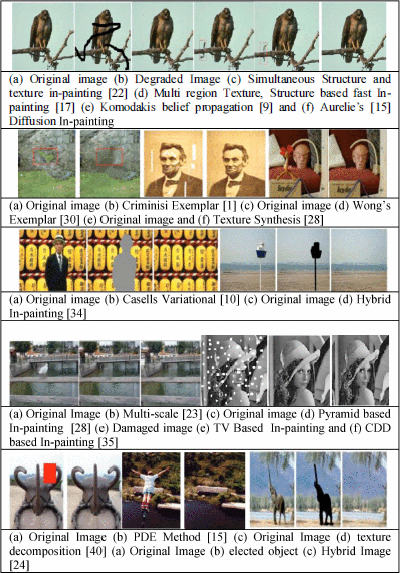
\includegraphics[width=10cm]{assets/images/inpainting.png}
    \caption{
        \textbf{Príklady dokreslenia obrázkov rôznymi metódami \cite{6544390}.}
    }
    \label{fig:inpainting}
\end{figure}


% LOL - Toto neviem ci hej
% LRP sa taktiež ukázala ako pomerne robustná metóda pre overovanie správnosti modelu, pretože oproti iným metódam na interpretovanie neurónových sietí produkuje stabilnejšie výsledky pri opakovanom trénovaní modelu (tepelné mapy z LRP sú porovnávané po každej epoche s tou predchádzajúcou) \cite{esmaeilzadeh2018end}.

% \section{Výskumné tézy}

% \paragraph{Kombináciou existujúcich metód na interpretovanie a vysvetľovanie rozhodnutí neurónových sietí je možné zlepšiť interpretovateľnost / vysvetliteľnosť nerónovej siete predikujúcej Alzheimerovu chorobu.} Existujúce práce sa predovšetkým zaoberali porovnávaním jednotlivých metód interpretácia/vysvetľovania predikcie.

% \paragraph{Uplatnením interpretovateľnosti a vysvetliteľnosti neurónových sietí je možné vytvoriť podporný systém pre doktorov na diagnostiku Alzheimerovej choroby.} \citeauthor{bohle2019layer} uvádzajú LRP ako metódu na vysvetľovanie invididuálnych rozhodnutí neurónovej siete natrénovanej na diagnostiku Alzheimerovej choroby. Využitím (nielen) tejto metódy môžeme skúsiť vytvoriť podporný systém pre doktorov.

% \paragraph{Syntézou rôznych typov snímok je možné dosiahnuť presnejšie výsledky pri diagnóze Alzheimerovej choroby pomocou neurónových sietí.} Súčasné state-of-the-art riešenie \cite{esmaeilzadeh2018end} na dátovej množine ADNI využíva predovšetkým snímky z MRI, táto dátová množina avšak obsahuje aj snímky z PET. Využitím oboch typov snímkov môžeme skúsiť zlepšiť úspešnosť tohto modelu.

% % Mozne vyuzit LRP pri trenovani modelu

% \paragraph{Metóda LRP je využiteľná pri vysvetľovaní rozhodnutí neurónovej siete predikujúcej Alzheimerovuj chorobu zo snímkov pacientov s miernym kognitývnym poškodením (angl. mild-cognitive impairment).} \citeauthor{bohle2019layer} overovali metódu LRP na snímkoch pacientov s Alzheimerovou chorobou a zdravých jedincoch, túto metódu avšak neoverovali na pacientoch s miernym kognitývnym poškodením, čo diskutujú v závere ako možnú oblasť výskumu pre ďalšie štúdie.

% \paragraph{Metódy interpretovateľnosti neurónových sietí je možné využiť na určenie správnosti natrénovaného modelu (neurónovej siete natrénovanej na diagnostiku Alzheimerovej choroby).} \citeauthor{bohle2019layer} označili vedenú spätnú propagáciu ako metódu na zistenie oblastí snímku mozgu, na ktoré je neurónová sieť senzitívna. Porovnaním výstupu tejto metódy s mapou mozgu môžeme skúsiť určiť správnosť neurónovej siete, tj. či sa neurónová sieť rozhoduje na základe tých častí mozgu, ktoré sa v medicíne používajú na diagnostiku Alzheimerovej choroby.

\section{Zhrnutie}

Alzhemierova choroba je bez pochyby veľmi nebezpečnou chorobou, keďže nie je ''iba'' o strate pamäti ale patrí k častím príčinám smrti (Sek. \ref{sec:ad}). Diagnostika tejto choroby pozostáva najmä z neuropsychometrických testov a analýzy rádiologických snímkov (napr. z PET, MRI). V súčasnosti tieto rádiologické snímky posudzujú doktori samotný. Práve tu je priestor pre umelú inteligenciu, aby im pri posudzovaní týchto snímkov pomohla.

V doméne obrazových dát sa používajú najmä konvolučné neurónové siete, pretože majú veľmi dobrú schopnosť naučiť sa rozoznávať špecifické objekty z obrázka. Konvolučné neurónové siete sa v nižších vrstvách naučia rozoznávať jednoduchšie tvary/hrany a vo vyšších zložitejšie šruktúry až celé objekty. Keďže jednou z možností diagnostiky Alzheimerovej choroby je diagnstika pomocou rádiologických snímkov, je možné použiť neurónové siete práve pri detekcii tohto ochorenia.

Neurónovým sieťam sa doteraz podarilo dosiahnuť veľmi dobré výsledky pri detekcii Alzhemerovej choroby, niektoré state-of-the art riešenia dosahujú presnosť až \textbf{95.09\%} (\citeauthor*{suk2016deep} \citeyear{suk2016deep}). S takto vysokou úspešnosťou môžu byť veľmi dobrým pomocníkom doktorov. Do úvahy však musíme zobrať, že tieto výsledky boli dosiahnuté bez klasifikácie MCI pacientov. V reálnom svete doktora navštívia všetky typy pacientov - CN, MCI a AD. V tomto prípade neurónové siete dosahujú rádovo nižšiu presnosť (\textbf{61.1\%}, \citeauthor*{bohle2019layer} \citeyear{bohle2019layer}). Niektoré práce dosiahli tieto výsledky použitím informácií o veku a pohlaví pacienta. Keďže pravdepodobnosťou výskytu Alzheimerovej choroby po dovŕšení 85 rokov života je až 50\% (Sek. \ref{sec:ad}), je možné, že sa pri vyššom veku pacienta model začne rozhodovať najmä na základe tejto informácie a nie na základe obrazových dát. Zároveň to však môže neurónovej sieti pomôcť, ak nebude brať tento atribút ako hlavný indikátor Alzheimerovej choroby, ale skôr ako pomocný atribút, ktorý bude meniť jej správanie u rôznych typov pacientov. Tu je však dôležité, takúto neurónovú sieť podrobiť dôkladnou analýzou jej rozhodnutí. Osobne si ale myslím, že v produkčnom modeli by sa tento atribút mal vynechať. 

Ďaľším problémom neurónových sietí je, že sa správajú ako čierne skrinky. Preto je potrebné ich rozhodnutia interpretovať, aby bolo pre doktora zrejmé na základe čoho neurónová sieť urobila svoju predikciu. V tomto práve môžu pomôcť metódy na vysvetľovanie rozhodnutí neurónovej siete (tzv. white-box metódy), alebo iné black-box metódy.

Bežným používaním neurónových sietí ako pomocníka pre doktorov, nebráni len ich vysvetliteľnosť, ale aj ich schopnosť detekcie ochorenia, keďže aj tu je priestor na zlepšenie - napr. úspešnosti klasifikácie do CN, MCI a AD.

Pre pochopenie správania sa neurónových sietí poznáme metódy jej interpretovania a vysvetľovania jej rozhodnutí. Interpretovaním neurónovej siete zisťujeme, ako si napríklad neurónová sieť predststavuje jednu z tried, ktorú klasifikuje. Vysvetľovaním jej rozhodnutí zas zisťujeme na základe čoho neurónová sieť spravila svoje rozhodnutie, a teda ktoré zo vstupných vlastnosti pozorovania ju navideli k zaradeniu do určitej triedy. Niektoré z týchto metód (LRP a vedená spätná propagácia) už boli použité pri vysveľovaní rozhodnutí neurónových sietí detekujúcich Alzheimerovu chorobu, avšak zatiaľ len pri binárnej klasifikácii pacientov.

% TODO
% 1-3 strany
% Vlastnymi slovami zhrnut state of the art
% Aky je stav, ake su trendy
% Co ste si z analyzy zobrali pre svoju pracu -> vychodiska